\documentclass{article}
\usepackage[utf8]{inputenc}
\usepackage{textcomp}
\usepackage{booktabs,rotating,tabularx}
\usepackage{graphicx}
\usepackage[english]{babel}
\usepackage{caption}
\usepackage{float}
\usepackage{hyperref} % provides \url{}
\usepackage[shortlabels]{enumitem} % enumeration package

% page layout and margin
\usepackage[a4paper, margin=2.54cm]{geometry}

% list spacing
\usepackage{enumitem}
\setlist{topsep=2pt, itemsep=2pt, partopsep=2pt, parsep=2pt}
\def\arraystretch{2}
% Header & Footer
\usepackage{fancyhdr}
\pagestyle{fancy}
\lhead{Software Engineering 2 - RASD}

\begin{document}

% title section
\begin{titlepage}
  \centering
  {\normalsize
    Software Engineering 2 - Prof. Di Nitto Elisabetta \\
    Dipartimento di Elettronica, Informazione e Bioingegneria \\
    Politecnico di Milano \par
  }     \vspace{3cm}
  {\Huge \textbf{eMall - e-Mobility for All\\} } \vspace{1cm}
  {\large \textbf{RASD\\Requirement Analysis and Specification Document} \par} \vspace{1cm}
  {\normalsize *Delivery Date here* \par} \vspace{4cm}
  {\normalsize Giovanni De Lucia (10700658) \\ Lorenzo Battiston (10618906) \\  Matteo Currò (here person code)\par} \vspace{4cm}
  \begin{figure}[h]
    \centering
    \includegraphics[scale=0.3]{src/Logo_Politecnico_Milano.png}
  \end{figure} \vspace{0.5cm}
\end{titlepage}

\tableofcontents

\section{Introduction}\label{intro}
\subsection{Purpose}
The following document is the RASD for the eMall - e-Mobility for All system. It provides
a description of the system focusing on the requirements and specifications, developing scenarios and use cases
to specify what the system must do, how it will interact with the stakeholders and the constraints it is subject to.

\subsection{Scope}
With the higher focus on the impact of our urban and suburban travel on the environment and the higher accessibility of electric mobility, an increase of circulating electric vehicles can be observed.
\footnote{\url{https://www.eea.europa.eu/ims/new-registrations-of-electric-vehicles}} \footnote{\url{https://www.statista.com/statistics/1101415/number-of-electric-vehicles-by-type/}} \footnote{\href{https://www.eib.org/en/surveys/climate-survey/4th-climate-survey/hybrid-electric-petrol-cars-flying-holidays-climate.htm}{European Investment Bank Climate Survey}}
This increase concerns both private vehicles and goods transporting ones.
As a result of restrictions on fuel vehicle production and sell that will concern a large part of the world's population\footnote{\href{https://en.wikipedia.org/wiki/Phase-out\_of\_fossil\_fuel\_vehicles\#Places\_with\_planned\_fossil-fuel\_vehicle\_restrictions}{Places with planned fossil-fuel vehicle restrictions}}, the number of
electric vehicle is still set to increase. For these reasons, the main vehicle manufacturers have started making huge investments in electric mobility\footnote{\href{https://en.wikipedia.org/wiki/Electric\_car\#EV\_plans\_from\_major\_manufacturers}{EV plans from major manufacturers}}, which will lead to greater accessibility to the market by drivers.\\
A main problem of electric vehicles is that a full charge requires much more time than a fuel vehicle refuel.
\footnote{\href{https://blinkcharging.com/fact-from-fiction-the-real-reason-why-consumers-dont-buy-electric-vehicles/?locale=en}{Why consumers don't buy electric vehicles}}
Thus, a single charge can have a huge impact on our daily schedule, and it is necessary to plan wisely when and where to charge.
Furthermore, some electric vehicle owners don't have the proper equipment to recharge at home, or their vehicle discharges in the middle of the road and the driver doesn't have the possibility to go home to recharge.\\
To solve these problems is one of the main objective of the eMall - e-Mobility for All system.\\
This system aims to develop an efficient planning of the charging process of electric vehicles that limits the carbon footprint caused by people mobility needs.\\\\
The main actor in this system are the drivers and the CPOs - Charging Point Operators, who manage their charging columns, along with the DSOs - Distribution System Operator, in charge of distributing the energy.
The digital system eMall should provide three main features:
\begin{itemize}
    \item \textbf{Booking} allows EV owners to book a charge. The remote booking avoids interference
          in the daily schedule of the owners, and it includes a notification
          system that alerts owners when their reservation is going to start.
    \item \textbf{Charging} allows EV owners to charge an EV, remotely monitor their charging
          process and be notified at the end of the charge.
          Thanks to these features, owners have not anymore the need to
          physically go to the CP when they want to retrieve details of their charge.
    \item  \textbf{Managing an EVCP} allows CPOs to get statistics on live and historical details
          about their EVCP - Electric Vehicle Charging Pool, to acquire information about the current energy price by
          DSOs and to decide in an automated way where to get energy for charging.
\end{itemize}




\subsubsection{World phenomena}
\begin{table}[H]
    \begin{tabularx}{\textwidth}{cX}
        \toprule
        \textbf{WP1} & An EV driver arrives at a charging station             \\
        \textbf{WP2} & Someone owns an electric vehicle                       \\
        \textbf{WP3} & A charging station is connected to the electrical grid \\
        \textbf{WP4} & Some charging station has solar panels                 \\
        \textbf{WP5} & Some charging station has a storage battery            \\
        \textbf{WP6} & An EV battery discharges                               \\ \bottomrule
    \end{tabularx}
\end{table}
\subsubsection{Shared phenomena}
\begin{table}[H]
    \centering
    \begin{tabularx}{\textwidth}{c|X|c}
        \toprule
        ID            &                                                                                                                                                                       & Controlled by \\ \midrule
        \textbf{SP1}  & An EV driver books a charge at a certain charging station                                                                                                             & world         \\ \midrule
        \textbf{SP2}  & An EV driver search for a specific charging station                                                                                                                   & world         \\ \midrule
        \textbf{SP3}  & The system suggest to charge based on daily schedule, special offers and availability                                                                                 & machine       \\ \midrule
        \textbf{SP4}  & An EV driver starts the charging process                                                                                                                              & world         \\ \midrule
        \textbf{SP5}  & An EV driver receives a notification when the charging process is completed                                                                                           & machine       \\ \midrule
        \textbf{SP6}  & An EV driver pays for the charge                                                                                                                                      & world         \\ \midrule
        \textbf{SP7}  & The system shows to CPO the status of its charging station as amount of energy in batteries, number of vehicle being charged and for each the time left of the charge & machine       \\ \midrule
        \textbf{SP8}  & The system shows to CPO information about the DSOs                                                                                                                    & machine       \\ \midrule
        \textbf{SP9}  & A CPO decide to acquire energy from a certain DSO                                                                                                                     & world         \\ \midrule
        \textbf{SP10} & The system notifies an EV driver that the charging shift will begin shortly                                                                                           & machine       \\ \midrule
        \textbf{SP11} & An EV driver monitors the charging status                                                                                                                             & machine       \\ \midrule
        \textbf{SP12} & An EV driver deletes a reservation                                                                                                                                    & world         \\ \midrule
        \textbf{SP13} & A CPO decide to retrieve the historical reservations on its EVSEs                                                                                                     & world         \\ \midrule
        \textbf{SP14} & An EV driver retrieves the historical reservations                                                                                                                    & world         \\ \bottomrule
    \end{tabularx}
\end{table}

\subsubsection{Goal}
\begin{table}[H]
    \begin{tabularx}{\textwidth}{cX}
        \toprule
        \textbf{G1} & Allows EV - Electric Vehicle driver to plan efficiently their charging process                                   \\
        \textbf{G2} & Allows EV - Electric Vehicle driver to have a single application for all the processes involving
        the charge with a personalized experience based on the car and the user commitments                                            \\
        \textbf{G3} & Allows CPOs - Charging Point Operators to be reached by a large number of EV drivers looking for charging points \\
        \textbf{G4} & Provides smart managing of charging stations, including the register of reservations                             \\
        \textbf{G5} & Allows CPOs - Charging Point Operators to choose between contracts of energy providers and
        to determine the energy source mix                                                                                             \\ \bottomrule
    \end{tabularx}
\end{table}

\subsection{Definitions, Acronyms, Abbreviations}

\subsubsection{Definitions}
\begin{itemize}
    \item EVCP - Electric Vehicle Charging Pool, is a station with multiple CPs
    \item CP - a synonym of EVSE, is a single charging column with multiple connectors
    \item Connectors - is a charging socket which can be of different types (e.g. CCS2, Type2)
    \item OCPP - Open Charge Point Protocol \footnote{\href{https://www.openchargealliance.org/protocols/ocpp-201/}{OCPP Protocol}}, todo
\end{itemize}

\subsubsection{Acronyms}
\begin{table}[H]
    \begin{tabularx}{\textwidth}{cX}
        \toprule
        \textbf{RASD} & Requirement Analysis and Specification Document \\
        \textbf{eMSP} & Electric Mobility Service Provider              \\
        \textbf{EV}   & Electric Vehicle                                \\
        \textbf{CPO}  & Charging Point Operator                         \\
        \textbf{DSO}  & Distribution System Operator                    \\
        \textbf{CPMS} & Charging Point Management System                \\
        \textbf{EVSE} & Electric Vehicle Supply Equipment               \\
        \textbf{CP}   & Charging Point                                  \\
        \textbf{EVCP} & Electric Vehicle Charging Pool                  \\
        \textbf{GPS}  & Global Positioning System                       \\
        \textbf{API}  & Application Programming Interface               \\
        \textbf{OCPP} & Open Charge Point Protocol                      \\
        \textbf{OS}   & Operative System                                \\
        \bottomrule
    \end{tabularx}
\end{table}

\subsubsection{Abbreviation}
\begin{table}[H]
    \begin{tabularx}{\textwidth}{cX}
        \toprule
        \textbf{WPx} & x-World Phenomena        \\
        \textbf{SPx} & x-Shared Phenomena       \\
        \textbf{Gx}  & x-Goal                   \\
        \textbf{Dx}  & x-Domain Assumption      \\
        \textbf{Rx}  & x-Functional Requirement \\
        \textbf{Ux}  & x-Use Case               \\ \bottomrule
    \end{tabularx}
\end{table}

\subsection{Revision history}
Nothing here

\subsection{Reference Documents}
Assignment document A.Y. 2022/2023 ("Requirement Engineering and Design Project: goal, schedule and rules")


\subsection{Document Structure}
Nothing here

\section{Overall Description}

\subsection{Product perspective}

\subsubsection{Registration}
Einar is a driver of an electric vehicle that uses every day to go to his office. He decided to download the eMall app because he heard by a friend of him that he can discover all the charging points in the entire world, booking one, starting a charge and pay for the charge, entirely through the app. After having downloaded it, launches the app for the first time and select sign in button to register into the system. He provides all the personal data required to access in the system and accept to personalise his experience by selecting his car from a provided list of all the EVs. He submits his data and the system asks him to verify his account through email or phone number.
\subsubsection{Book a charge}
Edvar wants to plan a charge for the next days and uses the app to find and book a carghing station nearby his office. In the home of the app he selected the book button and fills the information about the date and the time slot available for him to charge and indicates the zone in the map to scan for available charging stations. After submitting the form, the home page will change according to his information and displays a map of the selected zone with the available charging stations to book. 

Each charging station, if selected, shows the information about the charging point operator, the types of connectors, the availability of them for the filtered period, the charging power at which the connector operates and the cost for recharging 1 kWh. Edvar selected the charging station with the fastest connector but with the lowest price. To book the charge he selected one connector that is available and indicates when he want to start the charge and when to finish. The app, because Edvar accepted to insert his EV model, knows how much time is needed to charge his car so suggested the optimal time to book for a charge (from 10% to 80% of charge). He can accept the suggested book range or override the suggestion and modify the range at his willing inside the availabilty of the connector.

\subsection{Product functions}
Nothing here

\subsection{User characteristics}
Nothing here

\subsection{Assumptions, dependencies and constraints}
Nothing here

\section{Specific requirements}

\subsection{External Interface Requirements}
In this section are described details about user interfaces, hardware and application programming interfaces.

\subsubsection{User Interfaces}
\begin{figure}[H]
    \subfloat[Details]{
        \includegraphics[scale=0.1]{src/mockups/details.png}
    }
    \subfloat[Booking]{
        \includegraphics[scale=0.1]{src/mockups/book.png}
    }
    \subfloat[Cost detail]{
        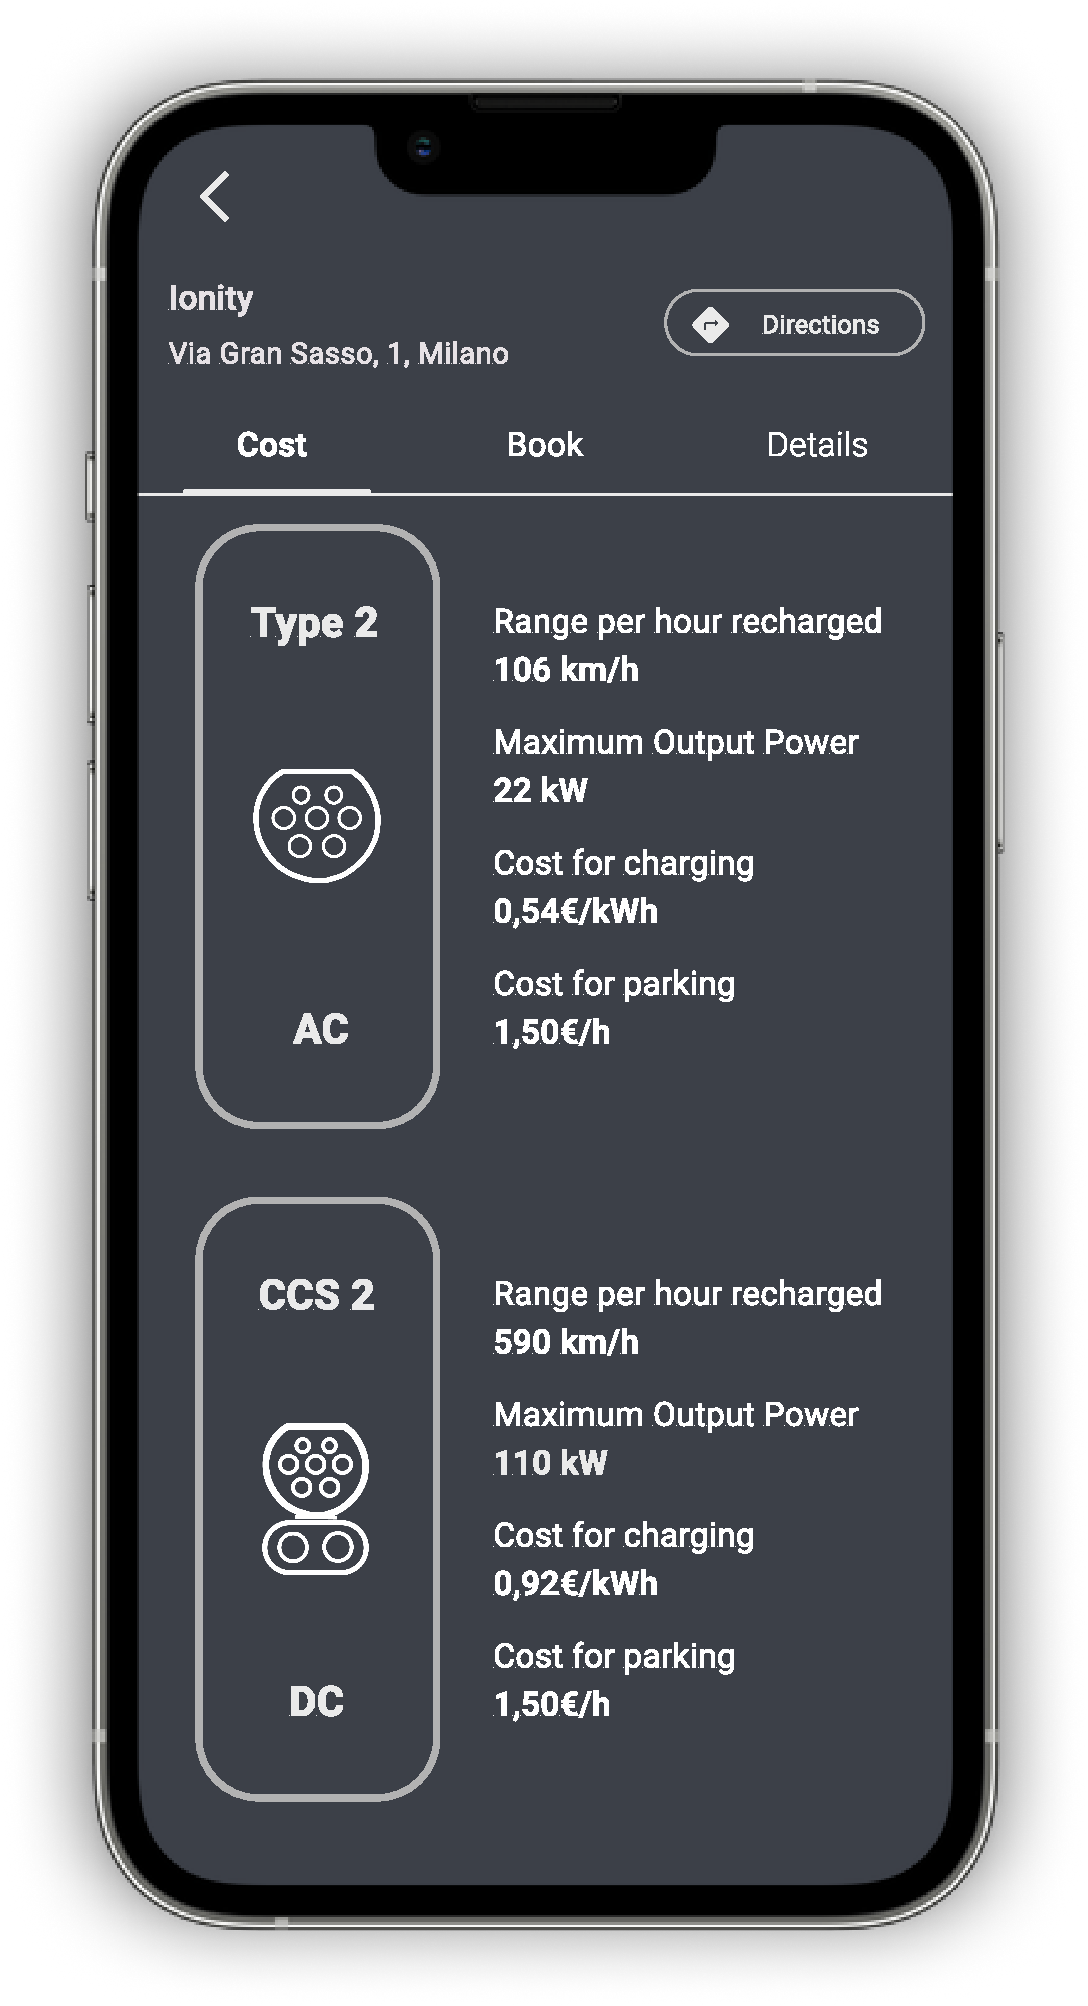
\includegraphics[scale=0.1]{src/mockups/book_cost.png}
    }
    \newline
    % following mockups
\end{figure}


\subsubsection{Hardware Interfaces}
Nothing here

\subsubsection{Software Interfaces}
Nothing here

\subsubsection{Communication Interfaces}
Nothing here

\subsection{Use cases}

\begin{figure}[H]
    \centering
    \includegraphics[scale=0.6]{src/use_case_diagram/driver_registration.png}
\end{figure}

\begin{figure}[H]
    \centering
    \includegraphics[scale=0.6]{src/use_case_diagram/cpo_registration.png}
\end{figure}

\begin{figure}[H]
    \centering
    \includegraphics[scale=0.5]{src/use_case_diagram/cpo.png}
\end{figure}

\begin{figure}[H]
    \centering
    \includegraphics[scale=0.6]{src/use_case_diagram/driver.png}
\end{figure}

\usecase
{EV driver registration}
{EV driver}
{EV driver clicks 'Sign Up' in the application homepage}
{
    \begin{enumerate}
        \item The system sends user the registration form
        \item Driver enters name, surname, birth date, telephone number and password. Then submits the data upon reading and accepting the Privacy Policy and the Terms of Service
        \item The system sends a SMS to driver through an API containing a secret code
        \item The driver submits the received verification code
        \item The system verifies the code and displays a success message
    \end{enumerate}
}
{A new EV driver account is created}
{
    \begin{itemize}
        \item A required registration field is missing when the form is submitted
        \item A wrong verification code is submitted
        \item The timeout of verification expires
    \end{itemize}
}
{
    All the exception are treated the same: the system will notify user with a human-readable message and the user is redirected to the homepage
}

\usecase
{CPO registration} % name
{CPO} % actor
{CPO clicks 'Sign Up' in the business dedicated application homepage} % entry condition
{ % event flow
    \begin{enumerate}
        \item The system sends operator the registration form
        \item Operator enters company name, VAT, IBAN, and password. Then submits the data upon reading and accepting the Privacy Policy and the Terms of Service
        \item The system processes the provided information and display a success message
    \end{enumerate}
}
{A new operator account is created} % exit condition
{ % exceptions
    \begin{itemize}
        \item A required registration field is missing when the form is submitted
        \item The operator is not associated to the given VAT
    \end{itemize}
}
{ % notes
    All the exception are treated the same: the system will notify operator with a human-readable message and the operator is redirected to the homepage
}

\usecase
{Check energy in batteries} % name
{CPO} % actor
{Authenticated CPO is in "Monitor status of EVCP" tab} % entry condition
{ % event flow
    \begin{enumerate}
        \item The operator choose a specific EVCP and clicks 'check energy in batteries'
        \item The system shows the battery status of the selected EVCP, if any
    \end{enumerate}
}
{The 'Check energy in batteries' chart is shown} % exit condition
{ % exceptions
    \begin{itemize}
        \item ...
    \end{itemize}
}
{ % notes
    ...
}

\usecase
{Monitor specific charging process} % name
{CPO} % actor
{Authenticated CPO is in "Monitor status of CP" tab} % entry condition
{ % event flow
    \begin{enumerate}
        \item The operator choose a specific EVCP and clicks "monitor specific charging process"
        \item The system shows a list of active charging process and ask operator to choose one
        \item The operator choose a specific active charging process from the list
        \item The system shows the details of the chosen charging process
    \end{enumerate}
}
{The details of the specific charging process are displayed} % exit condition
{ % exceptions
    \begin{itemize}
        \item ...
    \end{itemize}
}
{ % notes
...
}

\usecase
{Monitor aggregate charging process} % name
{CPO} % actor
{Authenticated CPO is in "Monitor status of CP" tab} % entry condition
{ % event flow
    \begin{enumerate}
        \item The operator choose a specific EVCP and clicks "monitor aggregate charging process"
        \item The system shows a chart with a detailed view of aggregate charging processes
    \end{enumerate}
}
{The aggregate charging process details charts are displayed} % exit condition
{ % exceptions
    \begin{itemize}
        \item ...
    \end{itemize}
}
{ % notes
...
}

\usecase
{View historical reservations} % name
{CPO} % actor
{Authenticated CPO is in "View reservations" tab} % entry condition
{ % event flow
    \begin{enumerate}
        \item The operator choose a specific EVCP, choose "historical reservation" tab, and sets a specific time frame
        \item The system shows the reservation details of the chosen EVCP during the chosen time frame
    \end{enumerate}
}
{The details of the historical reservations are displayed} % exit condition
{ % exceptions
    \begin{itemize}
        \item ...
    \end{itemize}
}
{ % notes
...
}

\usecase
{View active reservations} % name
{CPO} % actor
{Authenticated CPO is in "View reservations" tab} % entry condition
{ % event flow
    \begin{enumerate}
        \item The operator choose a specific EVCP, choose "active reservation" tab
        \item The system shows a list of active reservation for the chosen EVCP
    \end{enumerate}
}
{The details of the active reservations are displayed} % exit condition
{ % exceptions
    \begin{itemize}
        \item ...
    \end{itemize}
}
{ % notes
...
}

\usecase
{Choose DSO} % name
{CPO} % actor
{Authenticated CPO is in "Manage CPs" tab} % entry condition
{ % event flow
    \begin{enumerate}
        \item The operator choose a specific EVCP, choose "Choose DSO" tab
        \item The system provides a list of available DSOs
        \item The operator select one DSO among the available ones and submit their choice to the system
        \item The system shows a list of active reservation for the chosen EVCP
    \end{enumerate}
}
{The details of the active reservations are displayed} % exit condition
{ % exceptions
    \begin{itemize}
        \item ...
    \end{itemize}
}
{ % notes
...
}

\subsection{Functional Requirements}


\subsubsection{CPO Functional Requirements}
\begin{table}[H]
    \begin{tabularx}{\textwidth}{cX}
        \toprule
        \textbf{R1}  & The system must allow unregistered operator to register an account and its EVSEs                                                  \\
        \textbf{R2}  & The system must allow making a special offer                                                                                      \\
        \textbf{R3}  & The system must allow monitoring the charging process to infer when the battery is full                                           \\
        \textbf{R4}  & The system must allow retrieving details on the amount of energy available in its EVSEs batteries                                 \\
        \textbf{R5}  & The system must allow retrieving details on the number of vehicle being charged and for each vehicle the amount of absorbed power \\
        \textbf{R6}  & The system must allow retrieving details on the charge time left for each connected vehicle                                       \\
        \textbf{R7}  & The system must allow retrieving details on active and historical reservations on its EVSEs                                       \\
        \textbf{R8}  & The system must allow acquiring information from the DSOs about the current price of energy                                       \\
        \textbf{R9}  & The system must allow deciding from which DSO to acquire energy from                                                              \\
        \textbf{R10} & The system must dynamically decide where to get energy for charging (electrical grid, battery or a mixture)                       \\ \bottomrule
    \end{tabularx}
\end{table}
\subsubsection{eMSP Functional Requirements}
\begin{table}[H]
    \begin{tabularx}{\textwidth}{cX}
        \toprule
        \textbf{R11} & The system must allow unregistered users to register an account                                                     \\
        \textbf{R12} & The system must allow registered users to login                                                                     \\
        \textbf{R13} & The system must allow authenticated users to personalize their experience by providing information of their EV      \\
        \textbf{R14} & The system must allow users to search for EVSEs in the map                                                          \\
        \textbf{R15} & The system must show to the users EVSEs nearby their current position                                               \\
        \textbf{R16} & The system must allow retrieving details on a given EVSE regarding connector types supported and cost of the charge \\
        \textbf{R17} & The system must allow booking of an EVSE for a certain time interval                                                \\
        \textbf{R18} & The system must allow booking of an EVSE if and only if it is free for the specified time interval                  \\
        \textbf{R19} & The system must notify users when the charging shift is about to start                                              \\
        \textbf{R20} & The system must allow authenticated users to start the charge                                                       \\
        \textbf{R21} & The system must suggest users when to charge based on daily schedule, special offers and availability               \\
        \textbf{R22} & The system must allow authenticated users to monitor the charging status                                            \\
        \textbf{R23} & The system must notify authenticated users when the charging process is completed                                   \\
        \textbf{R24} & The system must allow authenticated users to pay for the charge                                                     \\
        \textbf{R25} & The system must allow authenticated users to delete a reservation                                                   \\
        \textbf{R26} & The system must allow authenticated users to view historical reservations                                           \\ \bottomrule
    \end{tabularx}
\end{table}

\subsubsection{Mapping on requirement}
\begin{table}[H]
    \begin{tabularx}{\textwidth}{XXX}
        \toprule
        \textbf{Goal} & \textbf{Requirements} & \textbf{Assumptions} \\ \midrule
        G1            & R1,R2,R3              & D1,D2,D3             \\
        G2            & esempio               & esempio              \\
        G3            & esempio               & esempio              \\ \bottomrule
    \end{tabularx}
\end{table}

\subsection{Performance Requirements}
Nothing here

\subsection{Design Constraints}
Nothing here

\subsubsection{Standards compliance}
Nothing here

\subsubsection{Hardware limitations}
Nothing here

\subsubsection{Any other constraint}
Nothing here


\subsection{Software System Attributes}
Nothing here

\subsubsection{Reliability}
Nothing here

\subsubsection{Availability}
Nothing here

\subsubsection{Security}
Nothing here

\subsubsection{Maintainability}
Nothing here

\subsubsection{Portability}
Nothing here

\section{Formal Analysis Using Alloy}
Alloy is a specification language for describing, designing, and verifying the behavior of complex systems.
The language is based on first-order logic, and has a mathematical foundation that allows for automated reasoning
about the correctness of designs.
\subsection{Objectives of the analysis}
The main goal of the formal analysis is to formally describe the domain and properties of the system to be.
This goal is reachable modelling and formally representing the following entities:
\begin{itemize}
    \item actors of the system to be;
    \item reservations
    \item status of a reservation;
\end{itemize}

\subsubsection{Reservation Model}
Description for the first model
\lstinputlisting[language=C, basicstyle=\ttfamily\footnotesize]{src/alloy/reservationModel.als}
\begin{figure}[H]
    \centering
    %\includegraphics[width=1\textwidth]{alloy/firstmodel.png} the image of the world
\end{figure}

\subsubsection{A title for the second model}
Description for the second model
\lstinputlisting[language=C, basicstyle=\ttfamily\footnotesize]{src/alloy/secondmodel.als}
\begin{figure}[H]
    \centering
    %\includegraphics[width=1\textwidth]{alloy/secondmodel.png} the image of the world
\end{figure}

\section{Effort Spent}
\subsection*{Pair working}
\begin{table}[H]
    \begin{tabular}{lr}
        \toprule
        \textbf{DD Structure analysis, overview architecture brainstorming} & \textbf{4h}   \\
        \textbf{Component Diagram}                                          & \textbf{5h}   \\
        \textbf{Runtime View}                                               & \textbf{8h}   \\
        \textbf{Database Entity Relationship Diagram}                       & \textbf{2h}   \\
        \textbf{Final Review}                                               & \textbf{2.5h} \\
        \bottomrule
    \end{tabular}
\end{table}

\subsection*{Giovanni}
\begin{table}[H]
    \begin{tabular}{lr}
        \toprule
        \textbf{Introduction section}                          & \textbf{1h}   \\
        \textbf{Deployment View}                               & \textbf{1.5h} \\
        \textbf{Review: ER Diagram}                            & \textbf{1.5h} \\
        \textbf{NFR Traceability}                              & \textbf{1h}   \\
        \textbf{Component Interfaces: diagram and description} & \textbf{2.5h}   \\
        \textbf{Design Choices description}                    & \textbf{0.5h} \\
        \bottomrule
    \end{tabular}
\end{table}

\subsection*{Matteo}
\begin{table}[H]
    \begin{tabular}{lr}
        \toprule
        \textbf{Requirements traceability} & \textbf{5h} \\
        \textbf{Component Diagram}         & \textbf{1h} \\
        \bottomrule
    \end{tabular}
\end{table}

\subsection*{Lorenzo}
\begin{table}[H]
    \begin{tabular}{lr}
        \toprule
        \textbf{User Interface Design} & \textbf{3h} \\
        \textbf{Development process and approach} & \textbf{1.5h} \\
        \textbf{Implementation Plan} & \textbf{1h} \\
        \textbf{Integration Plan} & \textbf{4h} \\
        \textbf{System Testing} & \textbf{0.5h} \\
        \bottomrule
    \end{tabular}
\end{table}

\section{References}
\begin{itemize}
    \item Software Engineering II course slides
    \item Use Case Diagrams were made using draw.io\\ \url{https://app.diagrams.net/}
    \item All other diagrams were made using StarUML\\ \url{https://staruml.io/}
\end{itemize}

\end{document}